\documentclass[10pt]{article}

\usepackage[utf8]{inputenc}
\usepackage[T1]{fontenc}
\usepackage{lmodern}
\usepackage[a4paper, margin=1.7cm, top=1.4cm, bottom=1.6cm]{geometry}
\usepackage{titlesec}
\titlespacing*{\section}{0pt}{0.9em}{0.35em}
\usepackage{amsmath, amssymb}
\usepackage{graphicx}
\usepackage{booktabs}
\usepackage{caption}
\usepackage{subcaption}
\usepackage{float}
\usepackage{microtype}
\usepackage{xcolor}
\usepackage{enumitem}
\usepackage{algorithm}
\usepackage[noend]{algpseudocode}
\usepackage{tikz}
\usetikzlibrary{arrows.meta, positioning, shapes.geometric}
\usepackage[hidelinks]{hyperref}

\captionsetup{font=small, labelfont=bf}
\setlength{\parskip}{0.3em}
\setlength{\textfloatsep}{0.6em}\setlength{\floatsep}{0.5em}\setlength{\intextsep}{0.5em}
\captionsetup{skip=3pt}
\setlength{\parindent}{0pt}
\setlist{itemsep=0.1em, topsep=0.2em}

\definecolor{accent}{RGB}{176,58,46}
\definecolor{boxbg}{RGB}{246,246,246}
\newcommand{\best}{\mathrm{best}}

\title{\textbf{Adaptive CEM Early Stopping:\\ An Inference-Time Extension to DINO-WM}\\[0.4em]
\large\textit{Reducing Planning Computation Through Convergence-Based Optimization}}
\author{EN4554 Deep Learning for Vision --- DINO-WM Reproduction Project}
\date{}

\begin{document}
\maketitle
\vspace{-3.6em}

\begin{center}
\fcolorbox{gray!60}{boxbg}{\parbox{0.94\linewidth}{\small
\textbf{Summary.} We implemented a convergence-based stopping rule for DINO-WM's CEM planner and
compared it with the original planner on 50 paired PointMaze tasks, using the same pretrained
checkpoint, tasks and seeds. Total CEM iterations fell by \textbf{51.3\%} and planning time by
\textbf{50.9\%}. Most of this saving comes from one task that the original planner failed. Without that task, the reductions are
\textbf{20.6\%} and \textbf{20.3\%} (95\% CI 8--31\%). Success was 49/50 for the original planner and
50/50 for Adaptive CEM. This difference is not statistically significant (McNemar $p{=}1.0$). On 39 of the 50 tasks, both planners did
identical work, because the original simulator-based success check ended planning first.}}
\end{center}

%%% =========================================================
\section{Motivation}

DINO-WM~\cite{zhou2024dinowm} plans at test time by optimising sequences of actions with the
Cross-Entropy Method (CEM)~\cite{rubinstein2004cem}. Each CEM iteration samples hundreds of candidate
action sequences and rolls every one through the pretrained world model. Planning cost therefore
grows linearly with the number of iterations, and the iteration budget is fixed in advance. If the
objective stops improving early, the remaining iterations still use GPU computation but change the plan very little.
We stop CEM once the best predicted cost has \emph{converged}. The method acts only at inference
time, so \textbf{no additional world-model training is required}, and the checkpoints and datasets are
unchanged. Stopping an optimiser when its objective stagnates is standard practice in the CEM
literature~\cite{rubinstein2004cem} and in sample-efficient CEM for control~\cite{pinneri2020icem}. We do not claim
novelty. Our contribution is to apply the rule to DINO-WM and measure its effect.

%%% =========================================================
\section{Original CEM Planning in DINO-WM}

For PointMaze, DINO-WM wraps CEM in Model Predictive Control (MPC). Each MPC step runs one CEM
\emph{planning call}, executes the first 5 world-model actions, and replans from the new state
(\texttt{conf/plan\_point\_maze.yaml}):

\begin{table}[H]
\centering\small
\begin{tabular}{lccccc}
\toprule
 & Candidates & Elites & Horizon & Max.\ iterations & Init.\ std \\
\midrule
Value & 300 & 30 & 5 WM steps & 10 & 1 \\
Config key & \texttt{num\_samples} & \texttt{topk} & \texttt{horizon} & \texttt{opt\_steps} & \texttt{var\_scale} \\
\bottomrule
\end{tabular}
\caption{CEM configuration for PointMaze. It is identical for both planners.}
\label{tab:baseline}
\end{table}

\textbf{Candidate evaluation.} At iteration $k$, $N{=}300$ sequences $a^{(n)}\sim\mathcal{N}(\mu_k,\sigma_k^2)$
are sampled, and the first sample is set to $\mu_k$. Each sequence is rolled out by the world model. Its cost is the mean-squared
distance between the predicted DINOv2 patch features at the final step and the goal features:
\begin{equation}
J\big(a^{(n)}\big) = \big\| \hat z_{H}^{(n)} - z_{g} \big\|_2^2 \,/\, D
\qquad(\texttt{objective.mode=last},\ \alpha{=}0).
\end{equation}
$\mu$ and $\sigma$ are then refitted to the 30 lowest-cost (elite) sequences.

\textbf{Existing early stopping.} With \texttt{eval\_every=1}, the current mean $\mu_k$ is executed in
the \emph{simulator} after every iteration. CEM stops as soon as the task is solved. This stop uses
ground-truth environment feedback. If the task is not solved, CEM runs all 10 iterations.

%%% =========================================================
\section{Proposed Adaptive CEM}

Let $C_k=\min_n J(a^{(n)}_k)$ be the lowest predicted cost found in iteration $k$. We track
\begin{equation}
C_k^{\best}=\min\!\big(C_{k-1}^{\best},\,C_k\big),
\qquad
r_k=\frac{C_{k-1}^{\best}-C_k^{\best}}{\max\!\big(|C_{k-1}^{\best}|,\,\delta\big)}\ \ (\ge 0),
\qquad
s_k=\begin{cases} s_{k-1}+1 & r_k<\tau\\ 0 & \text{otherwise}\end{cases}
\end{equation}
and stop when $k\ge K_{\min}$ and $s_k\ge P$. On a convergence stop, the planner returns the lowest-cost
sequence it actually evaluated, $a^\star$, rather than the refitted mean, which has not been evaluated. The original success
stop is unchanged and takes priority. Because $K_{\max}$ equals the baseline budget, the rule can only shorten
a planning call.

\begin{table}[H]
\centering\small
\begin{tabular}{lcll}
\toprule
Hyperparameter & Symbol & Config key (\texttt{planner.sub\_planner.adaptive\_cem.*}) & Value \\
\midrule
Enable adaptive stopping & -- & \texttt{enabled} (default \texttt{false}) & \texttt{true} \\
Minimum iterations & $K_{\min}$ & \texttt{min\_iterations} & 3 \\
Relative tolerance & $\tau$ & \texttt{relative\_tolerance} & 0.01 \\
Patience & $P$ & \texttt{patience} & 2 \\
Denominator guard & $\delta$ & \texttt{delta} & $10^{-8}$ \\
Maximum iterations & $K_{\max}$ & \texttt{opt\_steps} (existing) & 10 \\
\bottomrule
\end{tabular}
\caption{Adaptive CEM hyperparameters. These are initial experimental values and were \emph{not} tuned.}
\label{tab:hparams}
\end{table}

\begin{figure}[H]
\centering
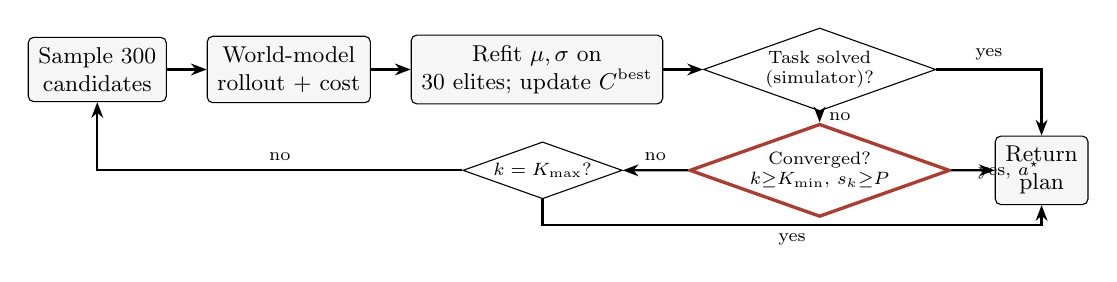
\begin{tikzpicture}[scale=0.92, transform shape,
  node distance=0.45cm and 0.55cm,
  box/.style={draw, rounded corners=2pt, fill=boxbg, align=center, font=\small, minimum height=0.8cm, inner sep=4pt},
  dec/.style={draw, diamond, aspect=2.8, fill=white, align=center, font=\scriptsize, inner sep=1pt},
  new/.style={dec, draw=accent, very thick},
  ar/.style={-{Stealth[length=2mm]}, thick}]
  \node[box] (s) {Sample 300\\candidates};
  \node[box, right=of s] (r) {World-model\\rollout + cost};
  \node[box, right=of r] (e) {Refit $\mu,\sigma$ on\\30 elites; update $C^{\best}$};
  \node[dec, right=of e] (succ) {Task solved\\(simulator)?};
  \node[new, below=0.15cm of succ] (conv) {Converged?\\$k{\ge}K_{\min},\,s_k{\ge}P$};
  \node[dec, left=0.9cm of conv] (max) {$k=K_{\max}$?};
  \node[box, right=0.6cm of conv] (out) {Return\\plan};
  \draw[ar] (s) -- (r);
  \draw[ar] (r) -- (e);
  \draw[ar] (e) -- (succ);
  \draw[ar] (succ) -- node[right, font=\scriptsize]{no} (conv);
  \draw[ar] (succ) -| node[pos=0.25, above, font=\scriptsize]{yes} (out);
  \draw[ar] (conv) -- node[right, font=\scriptsize, pos=0.4]{yes, $a^\star$} (out);
  \draw[ar] (conv) -- node[above, font=\scriptsize]{no} (max);
  \draw[ar] (max) -| node[pos=0.25, above, font=\scriptsize]{no} (s);
  \draw[ar] (max.south) -- ++(0,-0.35) -| node[pos=0.25, below, font=\scriptsize]{yes} (out.south);
\end{tikzpicture}
\caption{CEM loop with the added convergence check (red outline). All other blocks are the original planner.}
\label{fig:flow}
\end{figure}

%%% =========================================================
\section{Implementation}

The extension is implemented and backward compatible (Table~\ref{tab:status}). The world model, its
weights and the original evaluation results were not modified.

\begin{table}[H]
\centering\small
\begin{tabular}{p{0.30\linewidth}p{0.62\linewidth}}
\toprule
File & Change \\
\midrule
\texttt{planning/cem.py} & Optional per-instance convergence stop; best-so-far cost and sequence tracking; per-call instrumentation. \\
\texttt{conf/plan\_point\_maze.yaml} & Adds \texttt{adaptive\_cem} (disabled) and \texttt{stats\_filename: null}. \\
\texttt{experiments/adaptive\_cem/} & Task generator, paired runners, equivalence check, aggregation and plotting. \\
\bottomrule
\end{tabular}
\caption{Implemented changes. \texttt{mpc.py}, \texttt{evaluator.py}, \texttt{plan.py} and the models are unchanged.}
\label{tab:status}
\end{table}

\textbf{Convergence monitoring.} The planner reuses the existing \texttt{argsort} of the cost vector. $C_k$ is
\texttt{loss[topk\_idx[0]]}. $C^{\best}$, $s_k$, the stop flag and $a^\star$ are kept \emph{per instance}, and a converged
instance is frozen at $a^\star$ and skipped. In this experiment \texttt{n\_evals=1}, so every stop is per task.

\textbf{Instrumentation.} When \texttt{stats\_filename} is set, each CEM planning call appends one JSON record. It contains:
\begin{itemize}[leftmargin=1.2em]
\item the iterations executed and the stop reason (\texttt{success}/\texttt{converged}/\texttt{max\_iterations});
\item the candidates evaluated, and $C_k$, $C_k^{\best}$ and $r_k$ for every iteration;
\item batched world-model forward calls, counted with forward hooks that are paused during the simulator check;
\item planning time, measured with \texttt{time.perf\_counter} and \texttt{torch.cuda.synchronize}. It covers world-model inference and CEM
updates and excludes the simulator check, rendering, video writing and model loading.
\end{itemize}

\textbf{Verification.} With \texttt{enabled=false}, the planner gives bitwise-identical actions to the
original \texttt{git HEAD} code. On a toy world model this was checked for 1, 3 and 4 instances, with and without the success stop. On the real
checkpoint, the unmodified original code and the baseline mode were run on tasks 3 and 5. They produced identical logged metrics (maximum
absolute difference 0.0).

%%% =========================================================
\section{Experimental Methodology}

\textbf{Tasks.} With \texttt{n\_evals=1}, \texttt{plan.py} sets the task seed to $\texttt{seed}\cdot 0+1=1$ for every
run. As a result, our earlier 50 PointMaze reproduction runs all evaluated \emph{the same} start/goal pair, and that
evaluation cannot serve as a 50-task baseline. We generated 50 \emph{distinct} tasks with the same sampling procedure
as \texttt{plan.py} (seeds 1--50). Task 1 reproduces the earlier task bit for bit. Both planners load identical task files.
For each pair, the aggregation script checks that the file hash, the start/goal targets each planner received, the seed and the CEM
settings all match.

\textbf{Controls.} Both planners use the same checkpoint, objective, CEM size (Table~\ref{tab:baseline}), success
criterion (position within 0.5), GPU (RTX~5090 Laptop), fp32 precision, and seed (= task index). As a result, CEM sampling
noise is identical until the adaptive planner first stops early. The original configuration replans until the task
succeeds, so we cap MPC at 20 planning calls per task for both planners, and a capped task counts as a failure. Runs were
sequential, and the method order alternated between tasks.

\textbf{Metrics.} Every total includes \emph{all} MPC replanning calls. Reductions are computed from totals as
$R_X=(X_{\text{base}}-X_{\text{adaptive}})/X_{\text{base}}\times 100$, for iterations ($R_I$), planning time ($R_T$) and
candidates ($R_C$). Each has a 95\% bootstrap confidence interval (10{,}000 task resamples). For success, we
report the discordant pairs and an exact McNemar test.

%%% =========================================================
\section{Experimental Results}

\begin{table}[H]
\centering\small
\begin{tabular}{lccc}
\toprule
Metric (50 paired tasks) & Original CEM & Adaptive CEM & Change \\
\midrule
Successful tasks / success rate & 49 / 98.0\% & 50 / 100.0\% & +2.0 pp \\
Total CEM iterations & 452 & 220 & $-$51.3\% \\
Average CEM iterations per planning call & 5.72 & 3.10 & $-$45.8\% \\
Average MPC planning calls per task & 1.58 & 1.42 & $-$10.1\% \\
Total candidate sequences evaluated & 135{,}600 & 66{,}000 & $-$51.3\% \\
Total batched predictor forward calls & 2{,}260 & 1{,}100 & $-$51.3\% \\
Average planning time per task & 42.68\,s & 20.95\,s & $-$50.9\% \\
Total planning time & 2133.9\,s & 1047.7\,s & $-$50.9\% \\
Mean final state distance (position + velocity) & 4.700 & 4.551 & $-$3.2\% \\
\midrule
Stop reasons (planning calls): success / converged / max.\ iter. & 49 / 0 / 30 & 50 / 20 / 1 & \\
\bottomrule
\end{tabular}
\caption{Measured comparison on PointMaze. Planning time covers GPU-synchronised world-model inference and CEM updates.}
\label{tab:results}
\end{table}

\begin{table}[H]
\centering\small
\begin{tabular}{lccc}
\toprule
& $R_I$ (iterations) & $R_T$ (planning time) & $R_C$ (candidates) \\
\midrule
All 50 tasks & 51.3\% [11.1, 72.2] & 50.9\% [10.9, 71.9] & 51.3\% [11.1, 72.2] \\
Excluding task 45 (MPC cap hit) & 20.6\% [8.1, 31.4] & 20.3\% [7.8, 31.0] & 20.6\% \\
\bottomrule
\end{tabular}
\caption{Computation reductions with 95\% bootstrap confidence intervals.}
\label{tab:red}
\end{table}

\begin{figure}[H]
\centering
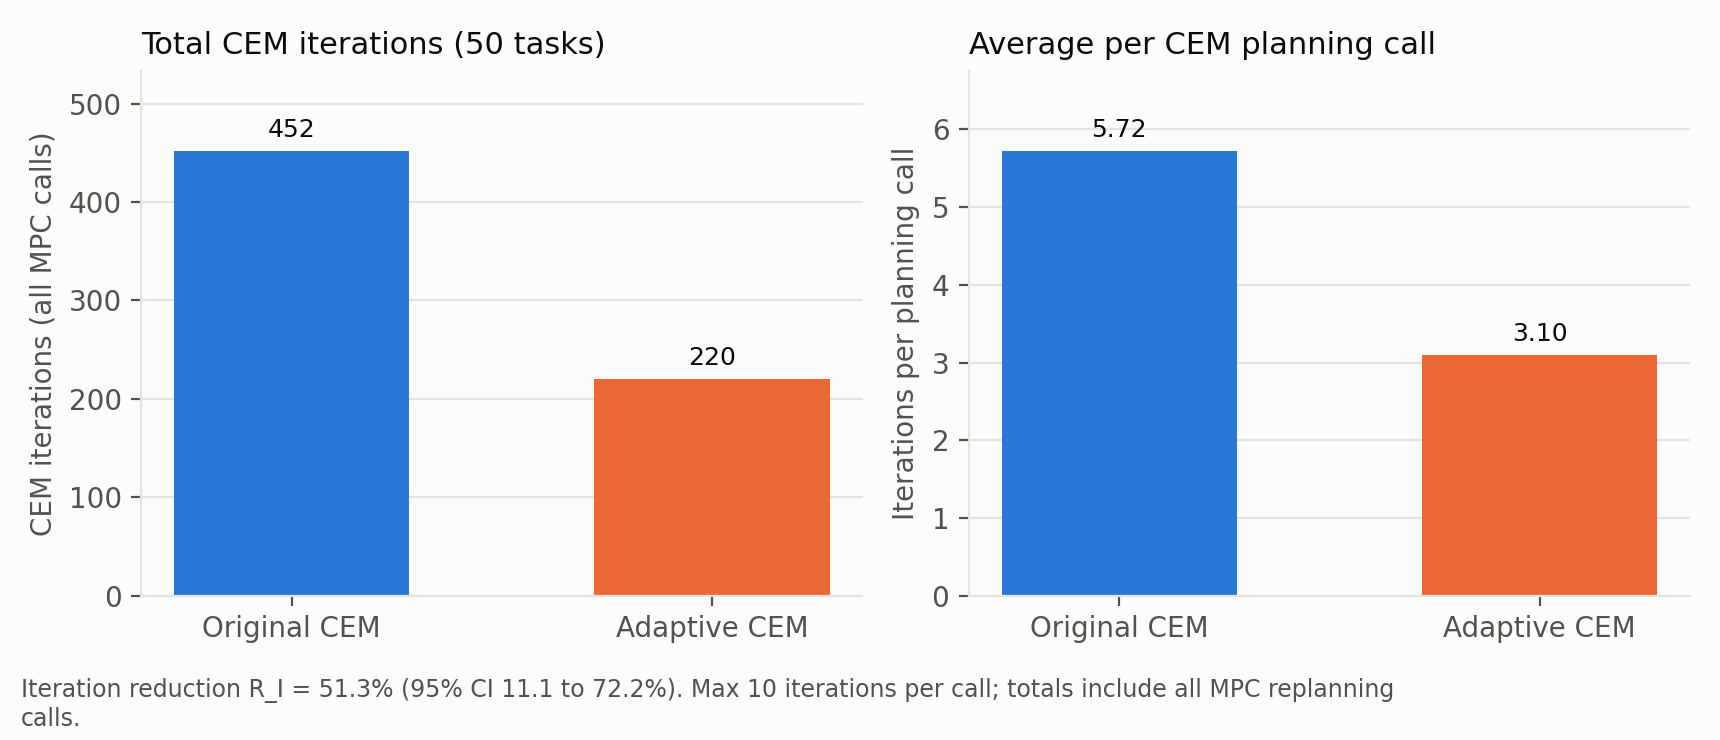
\includegraphics[width=0.49\linewidth]{figures/cem_iterations_comparison.png}\hfill
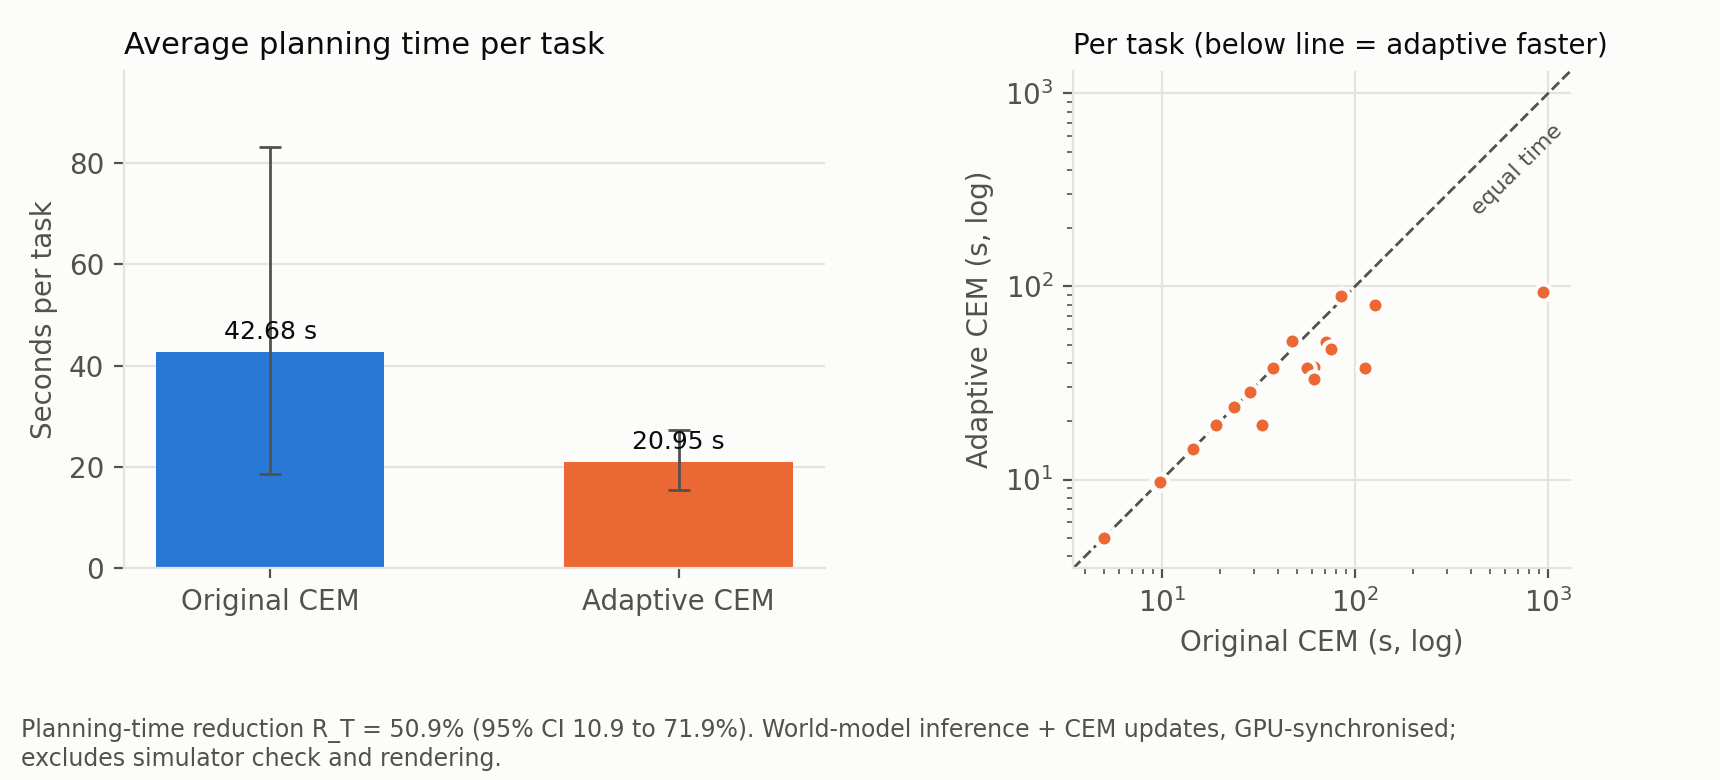
\includegraphics[width=0.49\linewidth]{figures/planning_time_comparison.png}
\caption{Left: total CEM iterations and average iterations per planning call. Right: average planning time per task
(95\% bootstrap CI) and per-task planning time on log axes. Points below the diagonal are tasks where Adaptive CEM was faster.}
\label{fig:totals}
\end{figure}

\begin{figure}[H]
\centering
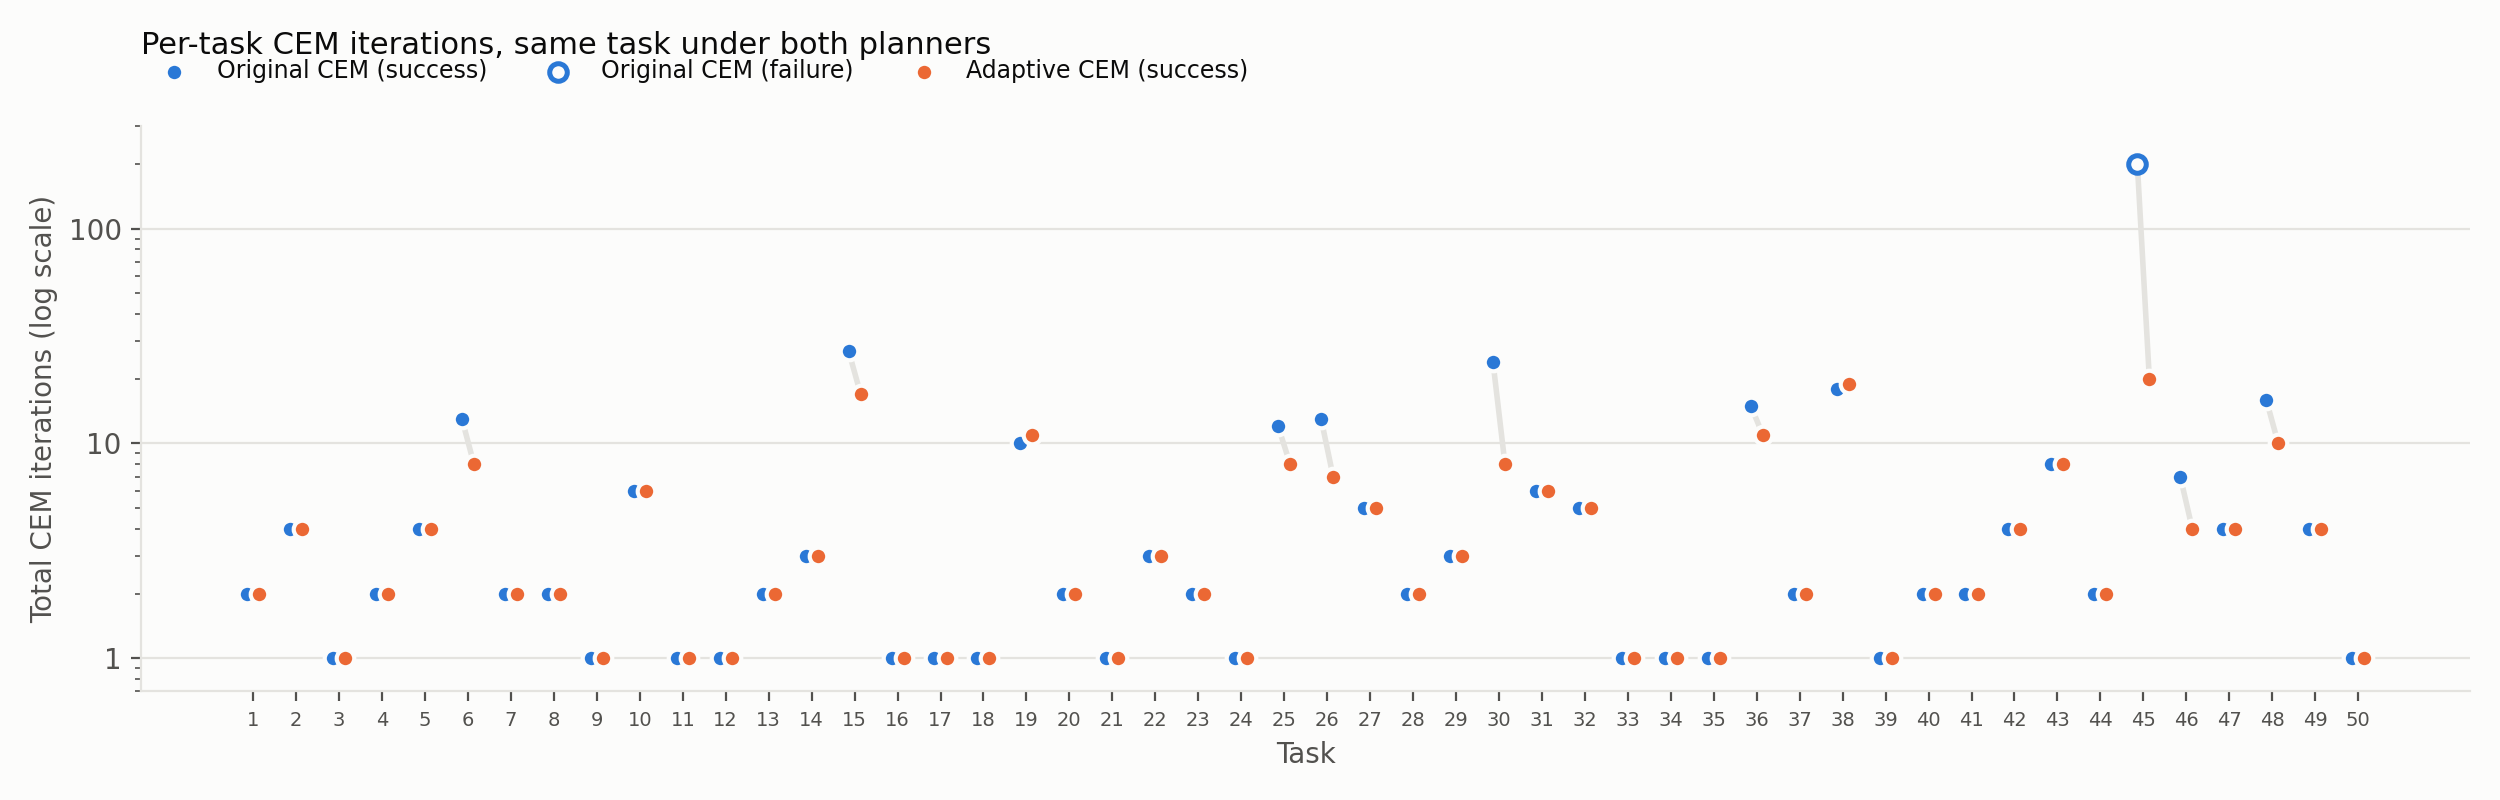
\includegraphics[width=\linewidth]{figures/per_task_iterations.png}
\caption{CEM iterations per task, summed over all MPC planning calls (log scale). Each task appears under both planners.}
\label{fig:pertask}
\end{figure}

\textbf{Where the savings come from.} Adaptive CEM used fewer iterations on 9 tasks, more on 2, and the same
number on 39 (Figure~\ref{fig:pertask}). The median per-task change in planning time is 0.00\,s. Convergence stops ended 20 of 71
planning calls after an average of 4.25 iterations (range 3--8). The original planner ran the full 10 iterations
in 30 calls. Task 45 dominates the totals. There, the original planner failed and hit the 20-call cap (200 iterations,
937.6\,s), while Adaptive CEM solved it in 4 calls (20 iterations, 94.1\,s). Table~\ref{tab:red} therefore also reports
results without this task. Stopping earlier increased MPC replanning on 7 tasks and reduced it on 2. This extra cost
is included in all totals. The cost per CEM iteration was essentially unchanged (4.72\,s vs.\ 4.76\,s), so the overhead of the
rule is negligible. Figure~\ref{fig:conv} shows a typical convergence stop.

\begin{figure}[H]
\centering
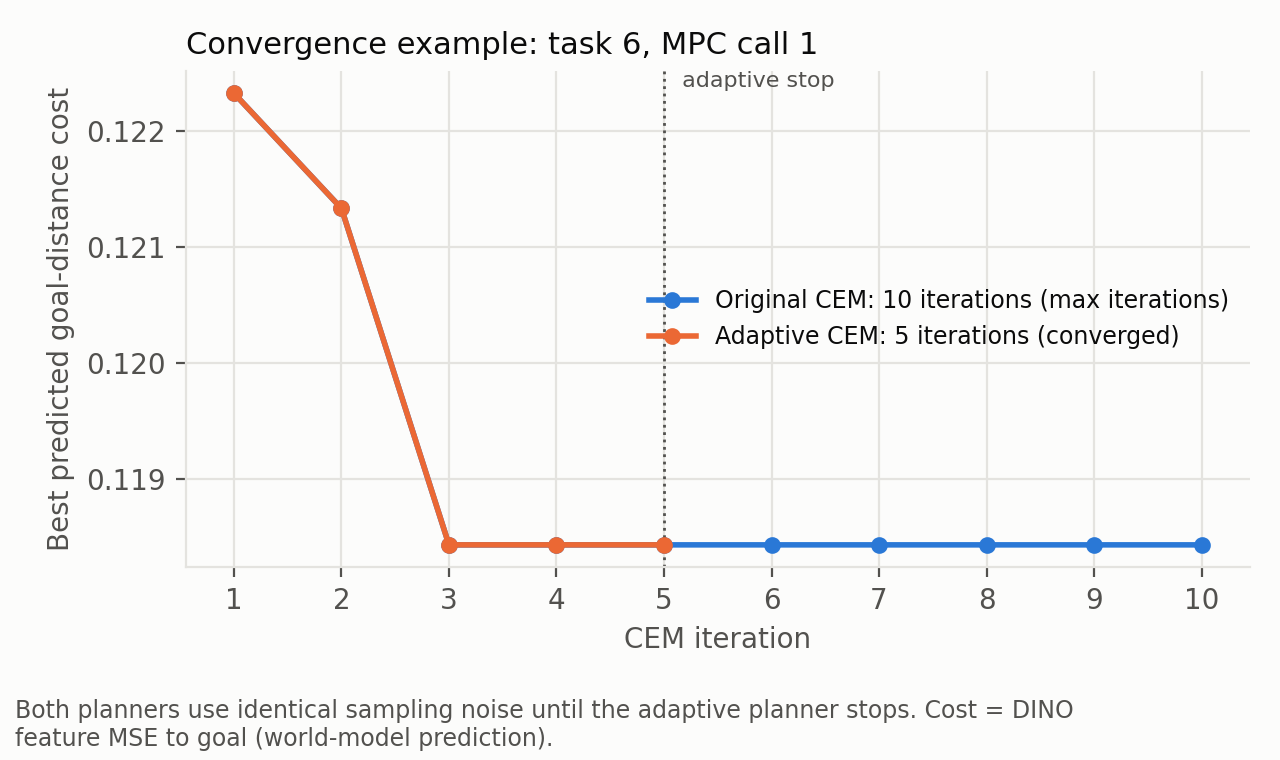
\includegraphics[width=0.56\linewidth]{figures/convergence_example.png}
\caption{Best predicted goal-distance cost in the first planning call of task 6. The cost plateaus at iteration 3. Adaptive
CEM stops after two iterations without improvement, while the original planner runs five more iterations with no gain.}
\label{fig:conv}
\end{figure}

%%% =========================================================
\section{Discussion and Conclusion}

\textbf{Computation.} Adaptive stopping reduced measured planning computation. Across all 50 tasks, $R_I{=}51.3\%$ and
$R_T{=}50.9\%$. The more representative figures, which exclude the one capped task, are $R_I{=}20.6\%$ and $R_T{=}20.3\%$. Both
confidence intervals exclude zero. The savings are concentrated in the harder tasks, where the original planner used all 10 iterations.

\textbf{Navigation performance.} Success was maintained in this sample: 49/50 for the original planner and 50/50 for Adaptive CEM, with one discordant
pair ($p{=}1.0$). The mean final state distance was similar. A single task is too little evidence to claim that adaptive
stopping \emph{improves} success, and 50 tasks cannot rule out small differences in either direction.

\textbf{Trade-offs.} An earlier stop can produce a less refined plan and require extra MPC replanning, as seen on 7 tasks. On
these tasks the net cost was still lower or similar. The original success stop uses \emph{privileged simulator feedback} and
ended most planning calls before the rule could act. This explains why 39 tasks were unaffected, and why Adaptive CEM
would likely matter more in a deployment setting without that oracle.

\textbf{Limitations and future work.}
(i)~The hyperparameters are untuned, and $\tau$ depends on the scale of the feature-space cost.
(ii)~Convergence is judged on the \emph{predicted} cost, so it inherits world-model errors.
(iii)~The study uses one environment and 50 tasks, the totals depend on the MPC cap, and timing comes from one GPU.
(iv)~The original planner re-encodes the start frame for all 300 candidates in each rollout. Caching that encoding is a separate,
orthogonal saving.
Future work: sweep $(\tau,P,K_{\min})$, evaluate without the simulator success check, and test on PushT and Wall.

\renewcommand{\refname}{\normalsize References}\vspace{-0.6em}
\begin{thebibliography}{9}\footnotesize\setlength{\itemsep}{0pt}\setlength{\parskip}{0pt}
\bibitem{zhou2024dinowm} G.~Zhou, H.~Pan, Y.~LeCun, L.~Pinto.
  DINO-WM: World Models on Pre-trained Visual Features enable Zero-shot Planning. \emph{arXiv:2411.04983}, 2024.
\bibitem{rubinstein2004cem} R.~Y.~Rubinstein, D.~P.~Kroese.
  \emph{The Cross-Entropy Method}. Springer, 2004.
\bibitem{pinneri2020icem} C.~Pinneri et al.
  Sample-efficient Cross-Entropy Method for Real-time Planning. \emph{CoRL}, 2020.
\end{thebibliography}

\end{document}
